\section{Modeling Seamless Branches}

\begin{flushleft}

Modeling the branches of a plant is the most important part behind the overall look and feel of that plant. The L-system described in the previous sections is able to describe the most important details about the plants structure. For instance the width, length, weight and other important information. Our job now is to take this information and intelligently generate a model consisting of vertices, normals, texture coordinates and other information that can then be provided to the GPU and then rendered on the screen.\\

\vspace{5mm}

The most obvious way to generate a model for a branching structure would be to take a number of cylinders and to rotate and stack them according to the branching structure. In this way we are able to represent the overall branching structure of the tree. However there is a problem pointed out by Baele and Warz\'{e}e "The branches junction causes a continuity problem: to simply stack up cylinders generates a gap" \cite{baele2005real}. This can be shown in the figure below:

\FloatBarrier

\begin{figure}[htbp]
	{\centering
		\vspace{7px}
		\setlength{\fboxrule}{1pt}
		\fbox{
			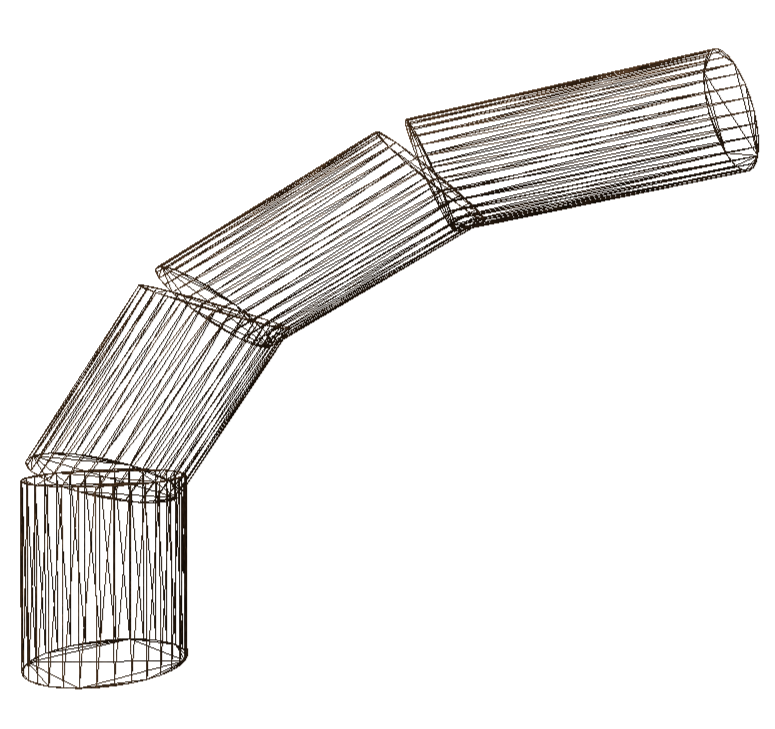
\includegraphics[scale=0.16]{Diagrams/stackedBranchesMesh.png}
		}
		\caption{Example of the continuity problem faced with stacked branching with a 25$^{\circ}$ bend per joint.}
	}
\end{figure}

\FloatBarrier

\vspace{5mm}


\vspace{5mm}

This simple method of stacking cylinders gives a reasonable looking tree structure and it is usually good enough when the angles of branches are not more than about 25$^{\circ}$ and the size of the branches do not change. However for a much more convincing tree structure we will want to do better than this. The logical next step would be to actively link the branch segments together.

\FloatBarrier

\begin{figure}[htbp]
	{\centering
		\vspace{7px}
		\setlength{\fboxrule}{1pt}
		\fbox{
			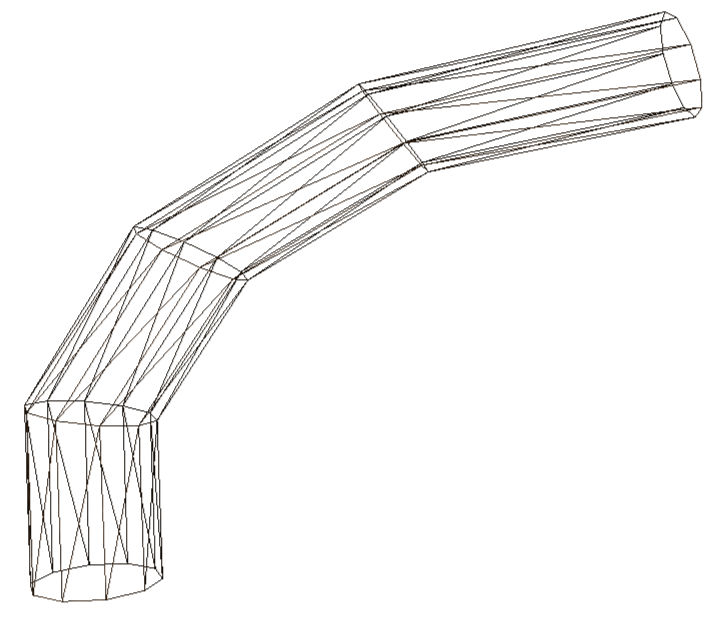
\includegraphics[scale=0.16]{Diagrams/linkedBranchesMesh.png}
		}
		\caption{Example of linked branching with a 25$^{\circ}$ bend per joint.}
	}
\end{figure}

\FloatBarrier

\end{flushleft}